\documentclass[12pt]{article}
\usepackage[ngerman]{babel}
\usepackage{amsmath}
\usepackage[utf8]{inputenc}
\usepackage{hyperref}
\usepackage{algorithm,algpseudocode}
\usepackage{setspace}
\setstretch{1.5}
\usepackage[paper=a4paper,left=25mm,right=35mm,top=25mm,bottom=20mm]{geometry}
\usepackage{graphicx}
\usepackage{wrapfig}
\usepackage{pdfpages}

\hypersetup{
    colorlinks,
    citecolor=black,
    filecolor=black,
    linkcolor=black,
    urlcolor=black
}

\begin{document}

\renewcommand{\figurename}{Abb.}
\def\figureautorefname{Abb.}
\def\algorithmautorefname{Alg.}

\floatname{algorithm}{Alg.}

\renewcommand{\algorithmicrequire}{\textbf{geg.:}}
\renewcommand{\algorithmicensure}{\textbf{ges.:}}
\renewcommand{\algorithmicprocedure}{\textbf{prozedur}}
\renewcommand{\algorithmicfor}{\textbf{für}}
\renewcommand{\algorithmicdo}{\textbf{wiederhole}}
\renewcommand{\algorithmicend}{\textbf{ende}}
\renewcommand{\algorithmicrepeat}{\textbf{wiederhole}}
\renewcommand{\algorithmicif}{\textbf{wenn}}
\renewcommand{\algorithmicelse}{\textbf{sonst}}
\renewcommand{\algorithmicthen}{\textbf{dann}}
\renewcommand{\algorithmicreturn}{\textbf{gib zurück}}
\renewcommand{\algorithmicuntil}{\textbf{solange}} % for the classic do ... while
\renewcommand{\algorithmicwhile}{\textbf{solange}} % for the classic do ... while
\newcommand{\sei}{\textbf{sei }}


\includepdf[pages={1}]{res/deckblatt_erklaerung.pdf}

\tableofcontents
\thispagestyle{empty}
\clearpage

\section{Risikofaktor Navigationsgerät}
"`Wenn möglich, bitte wenden"\ auf der Autobahn. "`Jetzt links abbiegen"\ im Kreisverkehr. Navigationssysteme können Todesfallen oder Verursacher schwerer Unglücke sein. Denn die Menschen vertrauen ihnen oft blind. So zum Beispiel erging es einem 33-jährigen im niedersächsischen Einbeck. Denn als die Polizei an der Unfallstelle eintraf, bot sich ihnen ein kurioses Bild: Der Pkw steckte auf einer abwärtsführenden Fußgängertreppe fest. Jegliche Versuche des Fahrers, sein Fahrzeug zu befreien, blieben erfolglos. Bedanken darf sich dieser Mann, ebenso wie eine junge Frau, die aufgrund eines Tippfehlers in einem Ort 850km entfernt vom gewünschten Ziel eintraf, bei der allzu freundlichen Stimme aus der Mittelkonsole \cite{navi}. Darum ist es umso wichtiger, dass "`Navis"\ immer über aktuellste Kartendaten verfügen und auch ausgiebig auf Fehler geprüft werden. 
\\
Aber nicht nur detailreiche Straßeninformationen sind für ein gutes Navigationsgerät von Bedeutung. Denn die Daten können noch so genau sein; wenn das Gerät keine vernünftigen Wege berechnen kann, ist es genau so unbrauchbar. Darum geht es in dieser Arbeit, nämlich die verschiedenen Methoden zur Wegberechnung in einem Straßen-\textit{Netz} oder ähnlichem. Es werden drei \textit{Algorithmen} vorgestellt und Vergleiche der selbigen angestellt, um festzustellen, für welche Zwecke welche Methode am zielführendsten ist. Als Werkzeug zur genaueren Untersuchung und für Vergleichsstatistiken habe ich zusätzlich ein Programm namens \textit{PathFinder} geschrieben, in dem die \textit{Algorithmen} adaptiert sind. Diese Ausführungen sind in gewisser Weise als Bedienungsanleitung des Programms zu sehen, da sich sämtliche Darstellungen und Tabellendaten darauf stützen. 
\\
Mit der Mathematik als Leitfach, im Themenbereich von Extremwertproblemen, wird konkret das \textit{Problem des kürzesten Wegs} in Angriff genommen. Der optimale, kürzeste Weg zeichnet sich aber nicht nur durch seine Eigenschaft, am schnellsten von \textit{A} nach \textit{B} zu gelangen, aus, sondern auch durch die für die Bestimmung dieses Wegs benötigte Zeit und den Rechenaufwand. Denn ein "`Navi", das vier Stunden rechnet, um den besten Weg zu ermitteln, wird sich nicht bei den Konsumenten durchsetzen, aber genauso wenig ein Gerät, welches den Fahrer ohne Rechenzeit über Feld- und Waldwege lotst. Es muss eine \textit{Balance zwischen Quantität und Qualität} gefunden werden. Und wo diese Mitte liegt, versuchen wir nun herauszufinden.
\newpage

\section{Grundlagen und Terminologie}
\label{sec:basics}
In diesem Abschnitt werden die grundlegenden Begriffe der Graphen-Theorie geklärt. Auch Fachbegriffe aus der Implementierung durch die Informatik werden erläutert.
\\
Generell sind \textit{Algorithmen} eine festgelegte Abfolge von Schritten um Daten zu verarbeiten. In der Informatik sind diese einzelnen Schritte Befehle.
\\
Die Graphen-Theorie dient als Basis dieser Ausführungen. Zentrale Bedeutung hat der namensgebende \textit{Graph} $G\; = (V,\,E)$, alternativ auch \textit{Netz} genannt, welcher aus einer Menge von \textit{Knoten} $V$ (von engl. "`Vertex") und einer Menge \textit{Kanten} $E$ (von engl. "`Edge") besteht.
\\
Zeichnerisch werden \textit{Knoten} als Punkte oder Kreise dargestellt; \textit{Kanten} als Verbindungslinien zwischen zwei \textit{Knoten}. Jede \textit{Kante} hat einen \textit{Startknoten} und einen \textit{Endknoten}. 
\\
Sobald sich keinerlei \textit{Kanten} in der Darstellung kreuzen, wird ein \textit{Graph} als \textit{planar} bezeichnet. Wenn von einer \textit{gerichteten Kante} die Rede ist, lässt sich diese als Pfeil interpretieren, da die Verbindung unidirektional gilt. Ebenso gibt es die \textit{gewichteten Kanten}, denen nicht nur zwei \textit{Knoten} zugeordnet werden, sondern zusätzlich noch ein Gewicht $w$ (von engl. "`Weight"), ein Zahlenwert, der als Kosten der Beziehung zwischen den beiden \textit{Knoten} gesehen werden kann.
\\
In der Wegfindung ist ein \textit{Weg} $P$ (von engl. "`Path") als geordnete Abfolge von \textit{Knoten} definiert. Da in der Regel jedes \textit{Knoten}-Paar nur einfach verbunden ist, reicht in der Implementierung diese Annahme aus.
\\
Visuell wird der \textit{Graph} durch einen \textit{Layout-Algorithmus} dargestellt, der allen \textit{Knoten} durch gewisse Berechnungen Positionen zuteilt (vgl. \autoref{sec:layout}).
\\
Um ein \textit{Netz} zu generieren, wird eine Zufallsfunktion verwendet. Hierzu wird ein standardisierter \textit{Pseudozufall}-Generator verwendet \cite{random}. Dieser generiert kaum oder nur schwer vorhersagbare Abfolgen von Zahlen und genügt für unsere Zwecke. Aufgrund der nicht echten Zufälligkeit wird ein sogenanntes \textit{Seed}-System benutzt, eine spezielle Zahl, mit deren Übergabe an den Generator stets die selbe Zahlenfolge erzeugt werden kann.
\newpage
\section{Aufbau und Bedienung des Programms \textit{PathFinder}}
\label{sec:manual}
Das selbstgeschriebene Programm \textit{PathFinder}, im eigentlichen Fokus stehend, fungiert sowohl als visuelle Möglichkeit der Darstellung von \textit{Graphen}, als auch als Quelle für Vergleichsdaten und Messungen in selbst erzeugten Szenarien. Geschrieben ist die Anwendung in der Programmiersprache \textit{Java} unter Verwendung der \textit{JavaFX}-Standardbibliothek \cite{javafx} und umfasst über 3000 Zeilen Code in 39 Quelldateien.\footnote{siehe Anhang: CD-ROM}
\begin{figure}[h!]
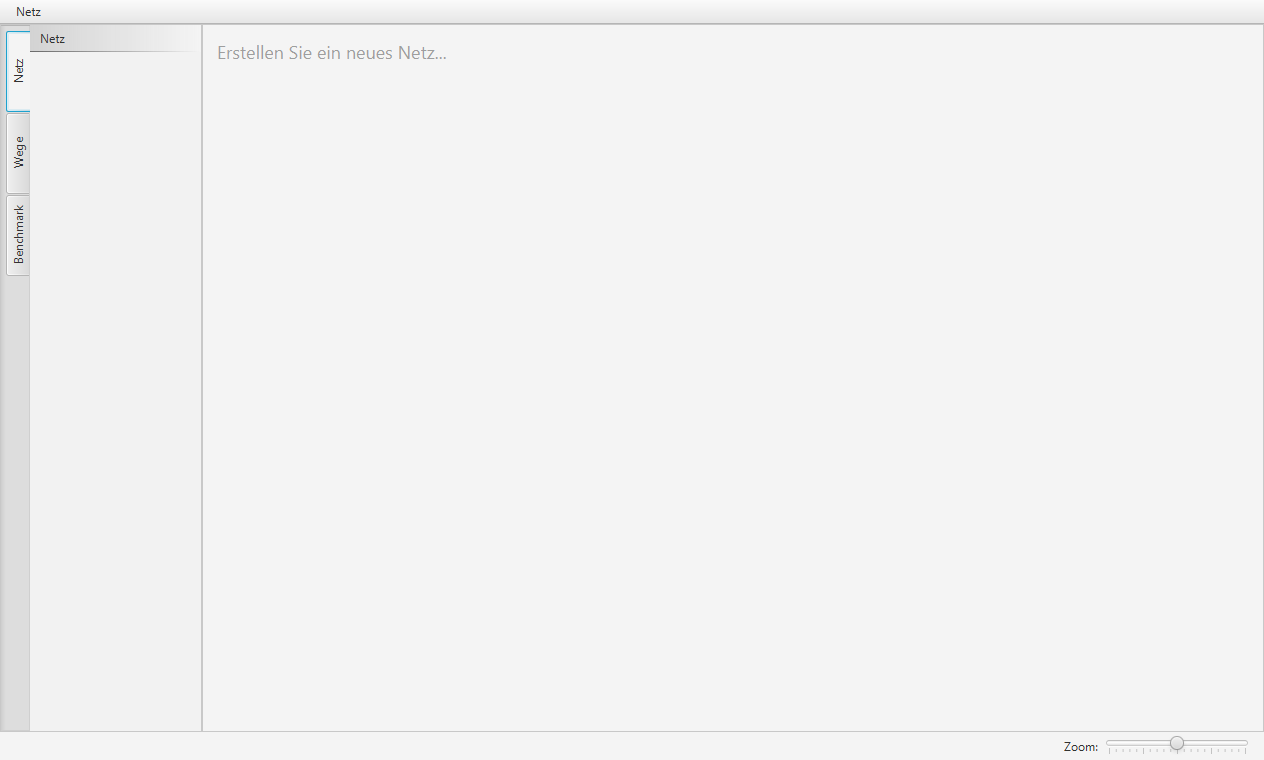
\includegraphics[width=0.8\textwidth]{res/main_screenshot.png}
\centering
\caption{Die Start- und Hauptansicht von \textit{PathFinder}}
\label{fig:main_screenshot}
\end{figure}
\\
Auf den ersten Blick ist die Anwendungsoberfläche in zwei größere Bereiche aufgeteilt. Im linken, kleineren Seitenbereich werden detaillierte Informationen über den \textit{Graphen}, bereits berechnete \textit{Wege} und die Konfigurationsmöglichkeiten neuer Wege, in mehreren "`Tabs"\ unterteilt, angezeigt. Der große rechte Bereich, zu Beginn der Anwendung nur mit "`Erstellen Sie ein neues Netz..." (\autoref{fig:main_screenshot}) beschriftet, dient als Hauptansicht von sowohl des \textit{Graphen}, als auch der Vergleichsstatistiken und Tabellen.
\\
Die Bedienung kann vollständig mit der Maus erfolgen, da sich sämtliche Features visuell intuitiv und minimalistisch präsentieren. Nur vereinzelt führen Tastatureingaben oder "`Hotkeys"\;zu mehr Komfort oder Genauigkeit der Anwendung. So kann beispielsweise das \textit{Relayout} (siehe \autoref{sec:layout}) des \textit{Graphen} per "`L"\ Taste, das \textit{Generieren} (siehe \autoref{sec:construct}) eines neuen \textit{Netzes} unter Benutzung von "`N"\ erfolgen.
\clearpage
\section{Konstruktion eines Graphen in \textit{PathFinder}}
\label{sec:construct}
Im nächsten Schritt wird nun ein Graph erzeugt und die Funktionsweise des Generators betrachtet. Durch Klicken auf "`Erstellen Sie ein neues Netz..."\ wird ein Dialog-Fenster geöffnet (\autoref{fig:new_graph_screenshot}), welches verschiedene Genererierungs-
\begin{wrapfigure}{l}{0.45\textwidth}
\vspace{-20pt}
\begin{center}
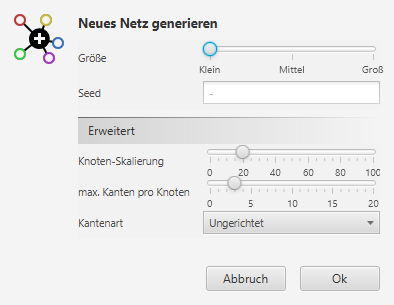
\includegraphics[scale=0.6]{res/new_graph_screenshot.png}
\end{center}
\vspace{-20pt}
\centering
\caption{Dialog zur \textit{Netz}-Generierung}
\label{fig:new_graph_screenshot}
\end{wrapfigure}
\textit{Parameter} zur Konfiguration anbietet. 
\\
Unterteilt sind diese Einstellungen in zwei Bereiche: \textit{Generell} und \textit{Erweitert}. \textit{Generelle} Optionen sind für den einfachen Gebrauch ausreichend mit einem Regler für die Größe $s$ und ein \textit{Seed}-Eingabefeld ausgestattet. Der \textit{Seed} wird verwendet, um die Möglichkeit zu haben, in späteren Tests mit dem gleichen \textit{Graphen} zu arbeiten.
\\
Im \textit{Erweitert}-Bereich lässt sich die Generierung aufs Genaueste einstellen. So können die Anzahl an Maximalknoten $n_{max}$ und die maximale \textit{Kanten}-Anzahl $e_{max}$ pro \textit{Knoten} festgelegt werden. Ebenso kann die Wahl zwischen drei Typen $t$ von \textit{Kanten} getroffen werden: \textit{Ungerichtet}, \textit{Gemischt} und \textit{Gerichtet}, was alle \textit{Kanten} des zu generierenden \textit{Graphen} betrifft. Die Option \textit{Gemischt} bewirkt, dass die Gerichtetheit jeder \textit{Kante} zufallsbedingt ist.
\\
Durch Bestätigen per Klick auf "`Ok" wird der Generator mit diesen \textit{Parametern} gestartet und ein \textit{Netz} erzeugt.
\\
Zunächst wird der \textit{Seed} für den Zufallsgenerator gesetzt. Danach wird aus den gegebenen Grenzwerten die tatsächliche Menge von \textit{Knoten} berechnet und in den \textit{Graphen} eingesetzt. Daraufhin wird für jeden \textit{Knoten} eine Anzahl an \textit{Kanten} bestimmt. Durch das "`Clampen", d.h Einzwicken, Eingrenzen, der Start- und Generierungswerte durch
\vspace{-20pt}
\begin{gather*}
e = max\Big(1,\,R\Big(0,\;min\Big(\dfrac{n}{2}-1,\,e_{max}\Big)\Big)\Big) \\
\left(\begin{aligned}
max(a, b) \to \text{Größere der beiden Parameter}\\
min(a, b) \to \text{Kleinere der beiden Parameter}
\end{aligned}
\right)
\end{gather*}
wird gewährleistet, dass der Generator nicht mehr \textit{Kanten} platzieren kann, als eindeutig möglich ist. Jetzt wird versucht, sämtliche \textit{Knoten} durch zufällige Wahl mit einem anderen \textit{Knoten} zu verbinden, wobei der jeweils gesuchte \textit{Knoten} weder der Ausgangsknoten selbst, noch ein bereits verbundener \textit{Knoten} sein soll. Sobald eine Kombination gefunden wurde, wird die 
\begin{algorithm}
\caption{\textit{Graph-Generator} \label{alg:generator}}
\begin{algorithmic}[1]
\Statex
\Require {Zufallsgenerator R, max. Kantengewicht $W_{max} = 30$}
\Ensure {Graph g}
\Statex
\Procedure{generiereGraph}{$seed$, $s$, $n_{max}$, $e_{max}$, $t$}
	\State setze Seed von $R$ zu $seed$
	\State \sei $n$ $R(n_{max}/2,\,n_{max}) * s$ \Comment Zufällige Anzahl im Interval $\big[n_{max}/2;\;n_{max}\big[$
	\State füge $n$ $Knoten$ zu $g$ hinzu
	\For {$i=0 \to n$}
		\State \sei $e$ $max(1,\,R(0,\;min(n/2-1,\,e_{max})))$
		\For {$j=0 \to e$}
			\State \sei $index$ $i$
			\Repeat 
			\State \sei $index$ $R(0,\,n)$
			\Until $index$ gleich $i$ oder $Knoten_i$ mit $Knoten_{index}$ verbunden
			\State \sei $e$ Kante von $Knoten_i$ zu $Knoten_{index}$, Gewicht $w = R(0, W_{max})$
			\If {$t =$ \textsc{Gemischt} oder $(t =$ \textsc{Gerichtet} und $R() > R())$} \State \Comment $R>R =$ Zufallstest
				\State setze $e$ gerichtet
			\EndIf
			\State füge $e$ zu $g$ hinzu
		\EndFor
	\EndFor
\EndProcedure
\end{algorithmic}
\end{algorithm}
entsprechende \textit{Kante} mit einem ebenfalls zufallsgenerierten \textit{Gewicht} erstellt. 
Dann wird auf Basis des \textit{Kanten-Typs} die Gerichtetheit bestimmt und schließlich wird die \textit{Kante} im \textit{Graphen} platziert (\autoref{alg:generator})\footnote{vgl. Anhang: GraphGenerator.java}.
\section{Visuelles Layout von Graphen}
\label{sec:layout}
In vorangegangen Abschnitten wurde das grundlegende Konzept eines \textit{Graphen} bereits dargestellt. Wenn man sich nun mit der optimalen visuellen Darstellung eines \textit{Graphen} auseinandersetzt, begibt man sich in die Thematik der \textit{Layouts} (von engl. "`Anordnung") eines \textit{Graphen}.
\\ 
Es gibt die verschiedensten Ansätze, zu einer übersichtlichen Visualisierung zu gelangen, darunter die \textit{force-directed algorithms} (von engl. "`kraft-gerichtet"\ oder "`kraft-basiert")\cite{force-directed}. Diese simulieren ein einem großen Molekül ähnelndes Konstrukt, in dem verschiedene \textit{Kräfte}, die von \textit{Knoten} und \textit{Kanten} ausgehen, aufeinander wirken. Das Ziel solcher Simulationen ist das \textit{mechanische Equilibrium}, die gegenseitige Aufhebung jeglicher wirkenden \textit{Kräfte}.\\
Vorteile dieser Methode sind die enorme Flexibilität der Simulation und die sehr zufriedenstellenden Resultate in Bezug auf die \textit{Planarität} des visualiserten \textit{Graphen}. Als Nachteil lässt sich die mitunter sehr lange Laufzeit der Berechnung sehen, die benötigt wird, um ein akzeptables Ergebnis zu erhalten; insbesondere bei sehr großen \textit{Netzen}.
\\
Bei dem in \textit{PathFinder} verwendeten \textit{Algorithmus} handelt es sich um den \textit{Fruchtermann-Reingold Algorithmus}, welcher 1991 von Thomas M. J. Fruchterman und Edward M. Reingold an der University of Illinois veröffentlicht wurde \cite{fruchterman}. Ihre Methode verfolgt die folgenden Prinzipien: 
\\
\indent 1. Verbundene \textit{Knoten} sollten nebeneinander liegen
\\
\indent 2. \textit{Knoten} sollten nicht zu nah beieinander platziert werden
\\
Der Algorithmus versucht außerdem, alle \textit{Knoten} $n$ gleichmäßig innerhalb eines
\begin{wrapfigure}{l}{0.35\textwidth}
\vspace{-20pt}
\begin{center}
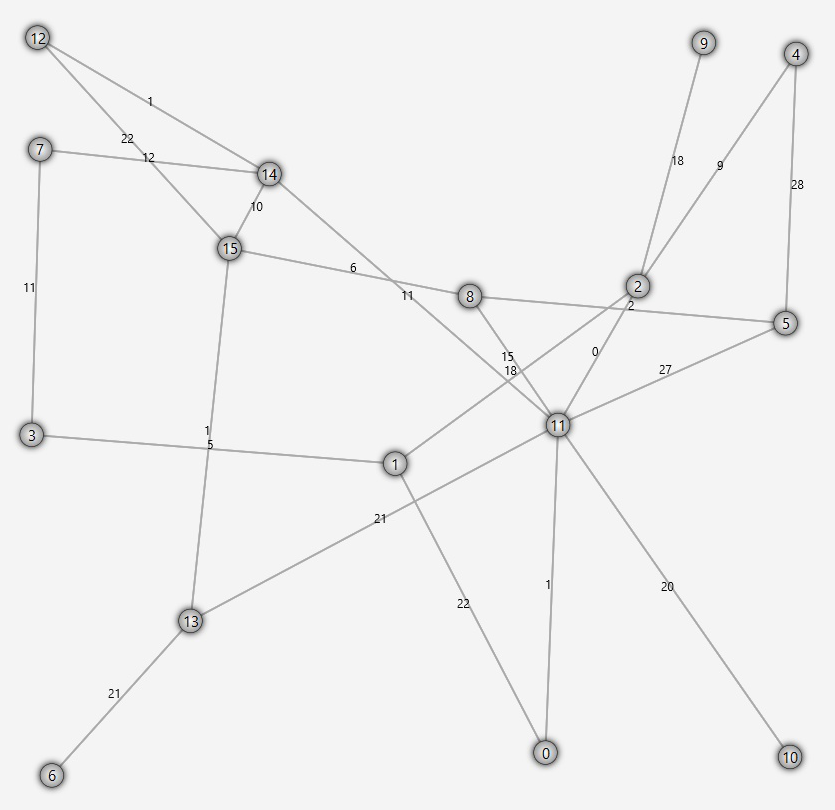
\includegraphics[scale=0.16]{res/graph_1.png}
\end{center}
\vspace{-30pt}
\centering
\caption{F.-R. Algorithmus}
\label{fig:graph_1}
\end{wrapfigure}
Rahmens zu verteilen, einer als Parameter $w$ und $h$ (von engl. "`width"\ und "`height") definierten Maximalfläche. Zunächst wird die Konstante $k$, die optimale Distanz zwischen \textit{Knoten}, als
\[
k = \sqrt{\dfrac{w \cdot h}{n}} 
\]
definiert. Sie findet Verwendung in den beiden \textit{Kräften} der Simulation. Die \textit{Kraft} $F_a$ beschreibt die Anziehung zwischen Knoten, $F_r$ die Abstoßung dieser voneinander.
\[
 F_a(x) = \dfrac{x^2}{k} \hspace{50pt} F_r(x) = \dfrac{k^2}{x}
\]
Der Ablauf der Simulation lässt sich in drei Schritte zusammenfassen. Zuerst wird $F_a$, danach $F_r$, für jeden einzelnen \textit{Knoten} berechnet. Im dritten Schritt werden die Effekte dieser berechneten \textit{Kräfte} umgesetzt (\textit{Disposition}), aber nur in durch die \textit{Temperatur} begrenzter Länge. Die \textit{Temperatur} ist ein Wert, der bei jedem Durchlauf des \textit{Algorithmus} bis auf $0$ verringert wird, um die Verschiebungen der \textit{Knoten} immer präziser werden zu lassen. Anfangs wird der Wert beliebig festgelegt. 
\newpage
\noindent Der vorgeschlagene und damit auch in \textit{PathFinder} umgesetzte Startwert $t_0$, dessen Änderung auf der Funktion $t(s)$ abgebildet wird, entspricht
\[
t_0 = \dfrac{1}{10} \cdot w \hspace{50pt} t(s) = t_0 \cdot \dfrac{s}{s_{max}} \hspace{50pt} s_{max} = s_g \cdot 500
\]
Außerdem wird eine Maximalanzahl $s_{max}$ an Simulationsschritten definiert, in deren Abhängigkeit die \textit{Temperatur} verringert wird. In der Anwendung wird diese Maximalgröße wie angegeben berechnet, wobei $s_g$ die bei der \textit{Graph}-Erzeugung angegebene \textit{Größe} ist.
\section{Wegfindungs-Algorithmen}
Nun folgt der eigentliche Hauptteil der Arbeit. Nachdem jetzt sowohl das Programm \textit{PathFinder}, als auch die darin angewandten Methoden zur Generierung und Visualisierung von \textit{Graphen} erläutert worden sind, wird nun auf die Wegfindung eingegangen.

\newpage

\subsection{Gröbste Züge von Intelligenz: Tiefensuche}
\begin{algorithm}
\caption{\textit{Tiefensuche} \label{alg:dfs}}
\begin{algorithmic}[1]
\Statex
\Require{Graph $G = (V,\ E)$}
\Ensure{Weg $P_{ab}$ von $n_a$ nach $n_b$}
\Statex
\Procedure{tiefenSuche}{$n_a$, $n_b$}
	\State markiere alle \textit{Knoten} in $G$ als $unbesucht$, außer $n_a$
	\State \sei $n$ aktiver \textit{Knoten} $n_a$
	\While{nicht alle \textit{Knoten} $besucht$ sind}
		\If{$n$ ist $n_b$}
			\State erschließe Weg $P_{ab}$ durch \textit{Vorgänger} und beende Suche
		\EndIf
		\If{$n$ keine unbesuchten Nachbarn hat}
			\State \sei $n$ \textit{Vorgänger} von $n$
		\Else
			\State sortiere unbesuchte Nachbarn von $n$
			\State \sei $n_{next}$ unbesuchter Nachbar mit geringstem \textit{Kantengewicht}
			\State setze $n$ als \textit{Vorgänger} von $n_{next}$
			\State \sei $n$ $n_{next}$
		\EndIf
	\EndWhile
\EndProcedure
\end{algorithmic}
\end{algorithm}
\newpage

\subsection{Heuristik als Mittel zum Ziel: Der Dijkstra-Algorithmus}
\begin{algorithm}
\caption{\textit{Dijkstra-Algorithmus} \label{alg:dijkstra}}
\begin{algorithmic}[1]
\Statex
\Require{Graph $G = (V,\ E)$}
\Ensure{Weg $P_{ab}$ von $n_a$ nach $n_b$}
\Statex
\end{algorithmic}
\end{algorithm}
\newpage
-
\newpage

\subsection{Der Allstar: Der A*-Algorithmus}
\begin{algorithm}
\caption{\textit{A*-Algorithmus} \label{alg:astar}}
\begin{algorithmic}[1]
\Statex
\Require{Graph $G = (V,\ E)$}
\Ensure{Weg $P_{ab}$ von $n_a$ nach $n_b$}
\Statex
\end{algorithmic}
\end{algorithm}
\newpage
-
\newpage

\section{Vergleichsstatistik und Fazit}
\newpage
\section{Schluss}
\newpage

%\nocite{*}
%\bibliographystyle{plain}
%\bibliography{WSeminar}
\begin{thebibliography}{9}
\bibitem{navi} vgl. Stern.de: Kuriose Navi-Unfälle\\
\newblock http://www.stern.de/digital/technik/navi-missgeschicke--in-100-metern-fahren-sie------in-den-fluss-3087618.html \\\emph{zul. abgerufen am 27.10.15}

\bibitem{random} Java Zufalls-Funktion\\
\newblock http://docs.oracle.com/javase/7/docs/api/java/util/Random.html \\\emph{zul. abgerufen am 18.10.15}
\bibitem{javafx} JavaFX-Homepage\\
\newblock http://docs.oracle.com/javase/8/javafx/get-started-tutorial/jfx-overview.htm \\\emph{zul. abgerufen am 14.10.15}

\bibitem{force-directed} Stephen~G. Kobourov\\
\newblock "`Spring embedders and force directed graph drawing algorithms.", 2012\\
\newblock http://arxiv.org/pdf/1201.3011v1.pdf \\\emph{zul. abgerufen am 24.10.15}

\bibitem{fruchterman} Thomas M.~J. Fruchterman and Edward~M. Reingold\\
\newblock "`Graph drawing by force-directed placement", 1991\\
\newblock ftp://ftp.mathe2.uni-bayreuth.de/axel/papers/reingold:graph{\_}drawing{\_}by{\_}force{\_}directed{\_}\\placement.pdf \\\emph{zul. abgerufen am 24.10.15}

\end{thebibliography}
\newpage


\includepdf[pages=2, pagecommand={\thispagestyle{plain}}]{res/deckblatt_erklaerung.pdf}
\end{document}
